\documentclass[es,practica,12pt]{uah}

\tema{7}
\titulo{Códigos Convolucionales}{Lesson title}
%
\begin{document}

\titulacion{Optativa GIEC y GIT}
\departamento{Teoría de la Señal y Comunicaciones}
\asignatura{Comunicaciones Digitales}{}
\curso{2021/2022}

\maketitle

\begin{abstract}
	Otro tipo de códigos correctores de errores son los códigos convolucionales, que veremos en esta práctica.
\end{abstract}

\section{Introducción}

Los códigos convolucionales son un tipo de códigos lineales, al igual que los códigos bloque, pero que en este caso obitienen la palabra código no sólo a partir de los bits de entrada actuales al codificador, sino también a partir de bits de información anteriores. Es decir, tienen memoria, lo que va a condicionar la forma de hacer la decodificación, que se realiza mediante el algoritmo de Viterbi. 

Los códigos convolucionales se utilizan en multitud de aplicaciones, incluyendo las comunicaciones móviles (GSM y 3G). 

En este caso vamos a utilizar funciones propias de Matlab para la codificación y decodificación, ya que la programación del algoritmo de Viterbi resulta especialmente complicada. 

\section{Desarrollo de la práctica}

\subsection{Ejemplo de los apuntes}
	\begin{enumerate}
	
		\item Vamos a reproducir el codificador de ejemplo que aparece en los apuntes del tema:
		%{\begin{figure*}[h!]\centering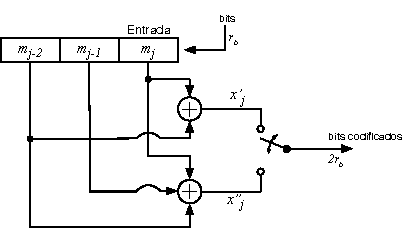
\includegraphics[width=10cm]{../Apuntes/Figuras/CodificadorConvolucional}\end{figure*}

		Como se puede ver en el esquema, se trata de un codificador que tiene un total de 2 retardos. El primer bit de salida se calcula a partir del bit actual y del bit de hace dos instantes de tiempo. Esto se puede codificar como que ese primer bit se calcula con una máscara que sería [\bits{1 0 1}], donde el primer 'bits{1}' representa que utilizamos el bit actual, el '\bits{0}' indica que no utilizamos el bit del instante anterior, y el último '\bits{1}' indica que sí que utilizamos el bit de hace dos instantes de tiempo. 

		De forma similar, el segundo bit de salida se obtiene a partir del bit actual, del bit anterior y de bit de hace dos instantes de tiempo. En este caso la máscara sería [\bits{1 1 1}]. 

		Con esto, vamos a utilizar la función \texttt{poly2trellis} que genera la representación del código convolucional a partir de dos parámetros:

		\begin{itemize}
				\item El número de instantes de tiempo que se consideran en el codificador (en nuestro caso, 3, el actual más los dos bits anteriores).
				\item Las máscaras que hemos visto antes para cada uno de los bits de salida, aunque convertidas a formato octal. En nuestro caso sería $[5 \, ,\, 7]$.
		\end{itemize}

		Ejecutad ese comando y guardad la configuración del codificador. Si abris la variable que devuelve esta función, podéis ver todos los parámetros del codificador: 
		\begin{itemize}
			\item Número de símbolos a la entrada: en nuestro caso son 2, es decir $log_2(2) = 1$ Bit
			\item Número de símbolos a la salida: en nuestro caso 4, es decir, $log_2(4) = 2$ bits. 
			\item Número de estados: El número de estados del codificador, que en este caso es 4 (podéis ver el diagrama de estados en los apuntes).
			\item Una matriz con el siguiente estado para cada posible estado actual y cada posible entrada.
			\item Una matriz con la salida para cada estado actual y entrada. 
		\end{itemize}
		
		\item Vamos a generar un vector de datos binario que coincida con la que se utiliza en los apuntes para el ejemplo de Viterbi: [\bits{1 1 0 1 0 1 0 0}].
		\item Nos queda ahora codificar ese vector de datos binarios con el codificador convolucional que hemos diseñado. Para eso utilizaremos la función \texttt{convenc}.
		\item Podéis observar la secuencia codificada y comprobar que coincide con la que se pone como ejemplo en los apuntes. 
		\item Vamos ahora a decodificar esta secuencia utilizando el algoritmo de Viterbi. Para ello utilizaremos la función \texttt{vitdec}. Toma cinco argumentos:
		\begin{itemize}
			\item Los datos que queremos decodificar
			\item La configuración del código convolucional que generamos al principio del todo.
			\item El número de bits transmitidos.
			\item El parámetro \texttt{'term'}, que indica que el decodificador empieza y termina en el estado cero. 
			\item El parámetro \texttt{'hard'}, que indica que a la entrada del decodificador hay bits en lugar de símbolos. 
		\end{itemize}
		Comprueba que la señal a la salida del decodificador coincide con los datos de entrada del principio. 

		\item Vamos a comprobar qué pasaría con una secuencia que tenga errores, como la del problema 2.12 de los apuntes: [\bits{1 0 1 0 1 0 0 1 0 1 0 1 0 1 1 1}]. Decodificad esta secuencia de bits y deberíais comprobar que la salida coincide con la secuencia de entrada a pesar de los errores. 
	\end{enumerate}

\subsection{Ejemplo más general}
	Una vez que hemos visto que el sistema funciona correctamente, vamos a utilizar una secuencia de bits más larga para poder extraer alguna conclusión de los resultados.

	\begin{enumerate}
		\item Generad una secuencia aleatoria de $10^4$ bits (podéis utilizar la función \texttt{randi} como en las prácticas anteriores).
		\item Codificad esa secuencia utilizando el mismo código convolucional que antes.
		\item Vamos ahora a pasar esa secuencia por un canal binario que introduce errores. Para ello podéis utilizar la función \texttt{bsc}. Utilizad una probabilidad de error de 0.01.
		\item Comprobad que el número de errores introducidos en la secuencia de bits da como resultado una probabilidad de error cercana a la marcada como objetivo.
		\item Ahora, decodificad la secuencia binaria recibida (la que tiene errores). En este caso es aconsejable utilizar la opción \texttt{'trunc'} en lugar de \texttt{'term'}, ya que aquí no tenemos garantizado que el sistema finalice en el estado cero. Con esta nueva opción se le dice que sí que empieza en el estado cero, pero analiza todos los caminos y elige el de mejor métrica global. 
		\item Comprobad la probabilidad de error final (en recepción) resultante. 
	\end{enumerate}

\subsection{Variación de la probabilidad de error}
	\begin{enumerate}
		\item Repetid el proceso del apartado anterior para probabilidades de error del canal de entre 0 y 0.1 en pasos de 0.001. Generad una gráfica con ejes semilogarítmicos en la que se compare el valor de la probabilidad de error del canal con el cociente entre la probabilidad de error real medida en recepción y la probabilidad de error del canal. Podéis representar la gráfica así: \texttt{semilogx(p, preal./p)}. Se debería obtener algo similar a esto:
		
		\centering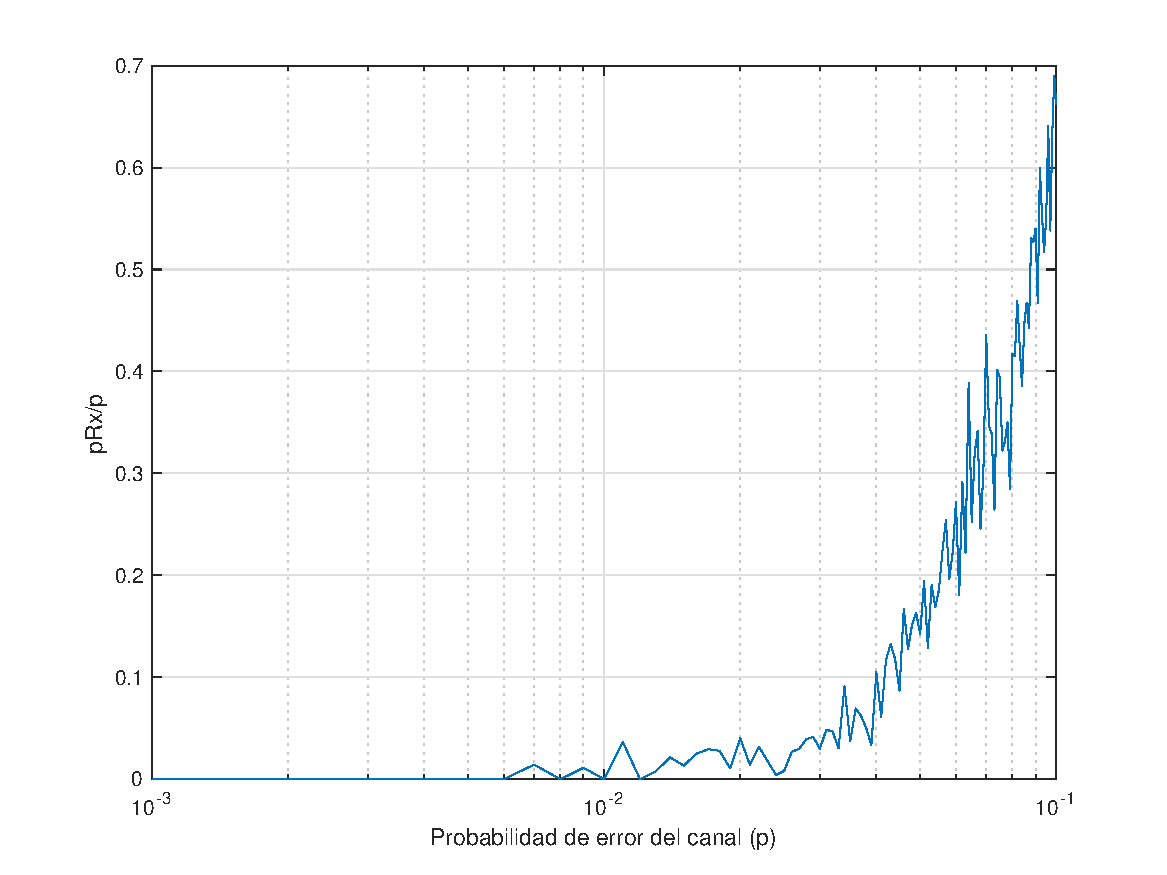
\includegraphics[width=8cm]{./Figuras/Figura1.pdf}
	\end{enumerate}


\subsection{Problema 2.11}
Intentad resolver el problema 2.11 de los apuntes utilizando el mismo procedimiento de antes. Comprobad que la salida del codificador coincide con la mostrada en la solución. 


\subsection{Complejidad computacional del algoritmo de Viterbi}
Uno de los problemas del algoritmo de Viterbi tiene que ver con su complejidad computacional. En concreto, si tenemos un codificador con $M$ estados y una secuencia de $T$ bits a la entrada, la complejidad computacional es del orden de $M^2 T$ y los requisitos de memoria dependen de $MT$. 

En primer lugar vamos a comprobar este dato. 

\begin{enumerate}
	\item Partiremos de nuevo del codificador de los primeros apartados de la práctica (el del ejemplo de los apuntes).
	\item Crearemos un bucle en el que iremos variando la longitud del vector de datos desde $10^4$ hasta $5\cdot10^6$ en pasos de $5\cdot 10^4$. 
	\item Para cada iteración, decodificaremos el vector de datos midiendo el tiempo que se requiere para ello (utilizad las funciones \texttt{tic} y \texttt{toc} de Matlab).
	\item Finalmente se debería obtener una gráfica similar a esta:
	
	\centering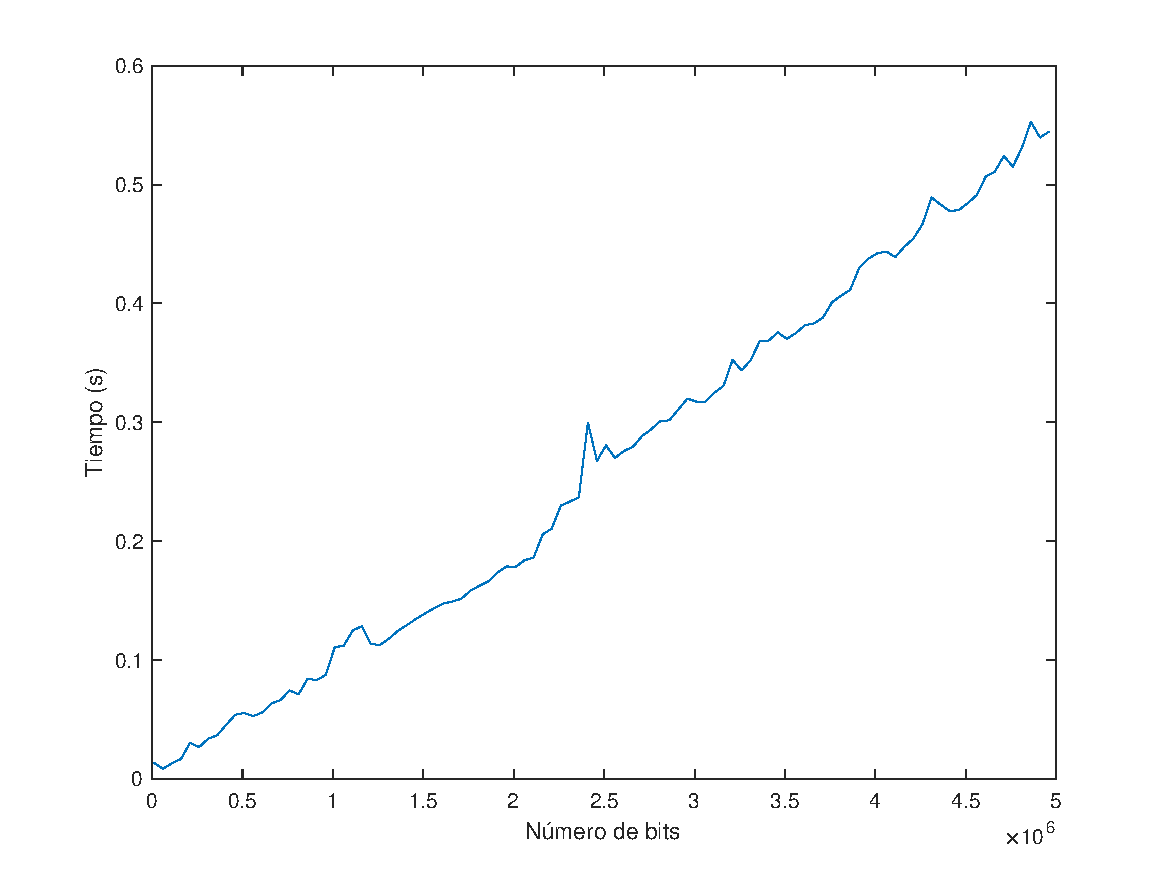
\includegraphics[width=8cm]{./Figuras/Figura2.pdf}
\end{enumerate}


\subsection{Ventana de decisión del algoritmo de Viterbi}

Tal cual está definido el algoritmo de Viterbi, es necesario esperar a disponer de todos los bits recibidos para obtener una decisión final sobre el primer bit recibido. Esto implica, por una parte, una excesiva necesidad de memoria en el sistema, y por otra, un retardo de codificación que no es aceptable en la mayor parte de los casos. 

Para evitar el problema anterior, lo que se hace es ``truncar'' la salida del sistema, de forma que se van tomando decisiones en base sólo a un número más recducido de bits, sin necesidad de esperar a toda la secuencia. Esto, no obstante, tiene como inconveniente que las prestaciones del sistema empeoran. Si el algoritmo de Viterbi se comporta como un receptor de máxima verosimilitud en condiciones óptimas, al hacer esto vamos a obtener una probabilidad de error algo peor. 

Para intentar comprobar este efecto, hagamos lo siguiente:

\begin{enumerate}
\item Partiremos una vez más del codificador convolucional que hemos utilizado en la mayor parte de los puntos de esta práctica. 
\item Para forzar a que el decodificador tome una decisión en base a un número limitado de bits a la entrada, modificad el comando, dejándolo así: \texttt{vitdec(yr,trellis,N,'cont','hard');}. Donde $N$ es el número de bits que utilizamos para la decisión, y que variaremos entre los valores $5$, $10$, $20$, $50$, $100$ e ilimitado (como en los apartados anteriores, con la opción \texttt{trunc}).
\item Construid un doble bucle, en el que se codifique una señal de $10^5$ bits con dicho codificador para cada uno de los valores de $N$ mencionados y considerando un canal con probabilidades de error $0.01, 0.02, 0.03, 0.04 y 0.05$. 
\item Representad la probabilidad de error medida en recepción frente a la probabilidad de error del canal para los distintos valores de $N$. Deberíais obtener algo parecido a esta figura:

\centering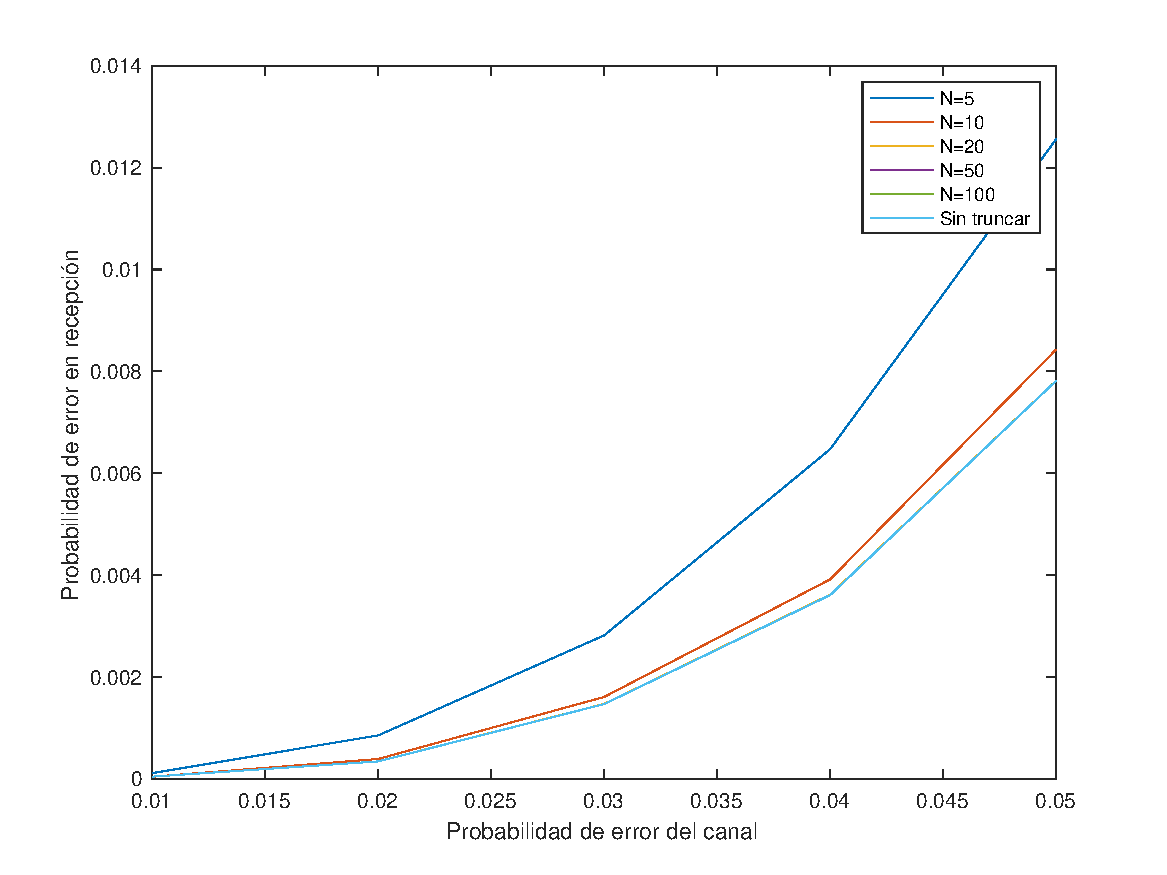
\includegraphics[width=8cm]{./Figuras/Figura3.pdf}
\end{enumerate}

\section{¿Qué entregar?}
\begin{itemize}
	\item Todas las funciones creadas.
\end{itemize}


%\printindex
\end{document}



	
